% !TeX root = ..\studio-operation-guide.tex
\section{Conference}

You can create a conference with other two parties using the phone's
local conference. You can create a conference between an active call and
a call on hold (on the same or another line) by pressing the
\scalerel*{
\includegraphics{images/yealink/btn-conference.png}}{B} key or
the \textbf{Conf} soft key.

\begin{quote}
	\textbf{Note}
	
	Network conference is not available on all servers. For more
	information, contact your system administrator.
\end{quote}

\subsection{Local Conference}

The SIP-T28P IP phone supports up to 3 parties (including yourself) in a
conference call.

This is the default method of conference called Local Conference.

\subsubsection{To set up a local conference call:}

\begin{enumerate}
	\item Place a call to the first party.
	\item When the first party answers the call, press
		\scalerel*{
\includegraphics{images/yealink/btn-conference.png}}{B} or the
		\textbf{Conf} soft key to place a new call.

		The active call is placed on hold.
	\item Enter the number of the second party and press
		\scalerel*{
\includegraphics{images/yealink/btn-ok.png}}{B},
		\scalerel*{
\includegraphics{images/yealink/btn-hash.png}}{B}, or the
		\textbf{Send} soft key.
		\begin{figure}[h]
			\centering
			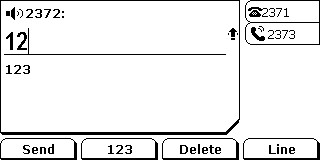
\includegraphics{images/yealink/screen-007.png}
		\end{figure}
	\item When the second party answers the call, you can consult with him or
		her before adding to the conference.
	\item Press \scalerel*{
\includegraphics{images/yealink/btn-conference.png}}{B}
		or the \textbf{Conf} soft key again to join all parties in the conference.
\end{enumerate}

\subsubsection{To join two calls in a conference:}

\begin{enumerate}
	\item Place two calls using two different accounts on the phone (for
		example, place the first call using account 1, and then place the
		second call using account 2).
	\item Press \scalerel*{
\includegraphics{images/yealink/btn-up.png}}{B} or
		\scalerel*{
\includegraphics{images/yealink/btn-down.png}}{B} to select
		the call for conference and ensure that the call is active (for example,
		select the call on account 1).
	\item Press \scalerel*{
\includegraphics{images/yealink/btn-conference.png}}{B}
		or the \textbf{Conf} soft key to join the two calls in the conference on
		the selected account.
\end{enumerate}

You can press \scalerel*{
\includegraphics{images/yealink/btn-hold.png}}{B}
or the \textbf{Hold} soft key to place the conference on hold. You can press the
\textbf{Split} soft key to split the conference call into two individual calls on
hold. To drop the conference call, press the \textbf{Cancel} soft key.

\subsection{Network Conference}

You can use network conference on the SIP-T28P IP phone to conduct a
conference with multiple participants.

This feature allows you to perform the following:

\begin{itemize}
	\item Join two calls together into a conference call.
	\item Invite another party into an active conference call.
\end{itemize}

To use this feature, contact your system administrator for the network
conference URI in advance.

\subsubsection{To set up a network conference call:}

\begin{enumerate}
	\item Place a call to the first party.
	\item Press \scalerel*{
\includegraphics{images/yealink/btn-conference.png}}{B}
		or the \textbf{Conf} soft key to place a new call.

		The active call is placed on hold.
	\item Enter the number of the second party and press 
		\scalerel*{
\includegraphics{images/yealink/btn-ok.png}}{B},
		\scalerel*{
\includegraphics{images/yealink/btn-hash.png}}{B}, or the
		\textbf{Send} soft key.
	\item When the second party answers the call, press
		\scalerel*{
\includegraphics{images/yealink/btn-conference.png}}{B} or
		the \textbf{Conf} soft key to add the second party to the conference.
	\item Press \scalerel*{
\includegraphics{images/yealink/btn-conference.png}}{B}
		or the \textbf{Conf} soft key to place a new call.

		The conference is placed on hold.
	\item Enter the number of the new party and then press 
		\scalerel*{
\includegraphics{images/yealink/btn-ok.png}}{B},
		\scalerel*{
\includegraphics{images/yealink/btn-hash.png}}{B},
		or the \textbf{Send} soft key.
	\item When the new party answers the call, press
		\scalerel*{
\includegraphics{images/yealink/btn-conference.png}}{B} or
		the \textbf{Conf} soft key to add the new party to the conference.
	\item Repeat steps 5 to 7 until you have added all intended parties.
\end{enumerate}

The procedures to set up a network conference call for specific servers
may be different from introduced above. Contact your system
administrator for more information.
